% Defence slide 10: what a conformal tower is, for a jury that has never met one.
% Two towers of boundary operators for the Ising class with free edges, drawn on a
% common axis of scaling dimension. Each tower is a primary plus descendants
% spaced by integers. The hollow marker at x=1 is the state that is absent.
% Colours match the tower slide in the results section.
\documentclass[tikz,border=3pt]{standalone}
\usepackage{amsmath,amssymb}
\usetikzlibrary{arrows.meta,decorations.pathreplacing}

\definecolor{ink}{RGB}{35,44,58}
\definecolor{towA}{RGB}{150,60,150}   % identity tower  (jwnnn)
\definecolor{towB}{RGB}{196,98,22}    % energy tower    (hl)

\begin{document}
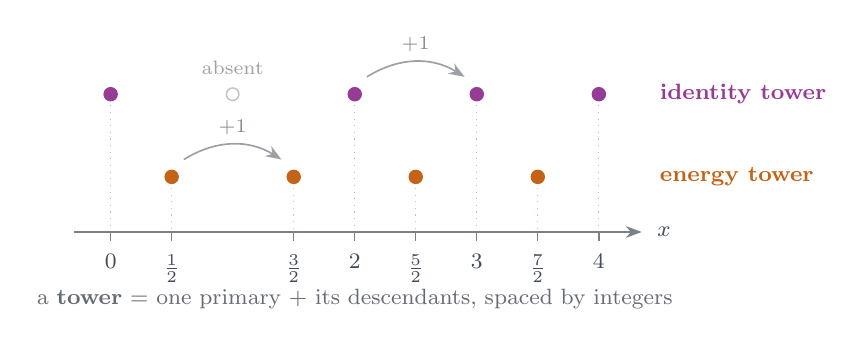
\begin{tikzpicture}[x=1.55cm, y=1cm,
    lab/.style={font=\footnotesize, color=ink!85},
    tag/.style={font=\footnotesize\bfseries},
    rise/.style={->, >=Stealth, line width=0.6pt, color=ink!45},
    dot/.style={circle, draw, fill, inner sep=1.7pt, line width=0.4pt}]

  % ---- identity tower: 0, (1 absent), 2, 3, 4 --------------------------------
  \def\ry{1.15}
  \foreach \x in {0,2,3,4} { \node[dot, towA, draw=towA] at (\x,\ry) {}; }
  \node[circle, draw=ink!30, fill=white, inner sep=1.6pt, line width=0.5pt]
    at (1,\ry) {};
  \node[lab, color=ink!45, anchor=south, font=\scriptsize] at (1,\ry+0.13)
    {absent};
  \node[tag, color=towA, anchor=west] at (4.42,\ry) {identity tower};
  \draw[rise] (2.10,\ry+0.22) to[bend left=32]
     node[midway, above, font=\scriptsize, color=ink!55] {$+1$} (2.90,\ry+0.22);

  % ---- energy tower: 1/2, 3/2, 5/2, 7/2 --------------------------------------
  \def\by{0.10}
  \foreach \x in {0.5,1.5,2.5,3.5} { \node[dot, towB, draw=towB] at (\x,\by) {}; }
  \node[tag, color=towB, anchor=west] at (4.42,\by) {energy tower};
  \draw[rise] (0.60,\by+0.22) to[bend left=32]
     node[midway, above, font=\scriptsize, color=ink!55] {$+1$} (1.40,\by+0.22);

  % ---- the shared axis of scaling dimension ----------------------------------
  \draw[->, >=Stealth, color=ink!60, line width=0.6pt] (-0.30,-0.60) -- (4.35,-0.60);
  \foreach \x/\t in {0/0, 0.5/{\tfrac12}, 1.5/{\tfrac32}, 2/2, 2.5/{\tfrac52},
                     3/3, 3.5/{\tfrac72}, 4/4} {
    \draw[color=ink!60, line width=0.5pt] (\x,-0.60) -- (\x,-0.72);
    \node[lab, anchor=north] at (\x,-0.76) {$\t$};
  }
  \node[lab, anchor=west] at (4.40,-0.60) {$x$};

  % dotted drop lines so each level reads against the axis
  \foreach \x in {0,2,3,4} { \draw[dotted, color=towA!45] (\x,\ry-0.14) -- (\x,-0.58); }
  \foreach \x in {0.5,1.5,2.5,3.5} { \draw[dotted, color=towB!45] (\x,\by-0.14) -- (\x,-0.58); }

  \node[lab, anchor=north, align=center, color=ink!70] at (2.0,-1.20)
    {a \textbf{tower} $=$ one primary $+$ its descendants, spaced by integers};
\end{tikzpicture}
\end{document}
